\documentclass{article}

\author{毛咏}
\title{基于Verilog和FPGA的多功能秒表设计实验报告}

\usepackage[fontset=ubuntu]{ctex}
\usepackage{indentfirst}
\setlength{\parindent}{2em}
\usepackage{graphicx}
\usepackage{listings}

\begin{document}
	\maketitle
    \tableofcontents
    \newpage
    
    \section{实验要求}
    
    	\par 1) 运用Verilog硬件描述语言,基于DE1-SOC实验板,设计实现一个具有较多功能的计时秒表。
        \par 2) 要求将8个数码管设计为具有“时:分:秒:毫秒”显示,按键的基本控制动作有3个:“计时复位”、“计数/暂停”、“显示暂停/显示继续”。功能能够满足马拉松或长跑运动员的计时需要。
        \par 3) 利用示波器观察按键的抖动,设计按键电路的消抖方法。
        \par 4) 在实验报告中详细报告自己的设计过程、步骤及Verilog代码。
	
	\section{设计思路}
    
    	\subsection{整体思路}
        	\par 毫秒部分每位满10进1,分秒低位满10进1,高位满6进1。计时按钮控制是否在时钟周期到达制定常数时加毫秒低位,显示按钮控制是否由变量改变导致高低电平变化,重置按钮控制变量清零以及计时与显示状态的复位。
            
    	\subsection{BDF设计}
        	\par 包含4个输入,一个是时钟脉冲,依据题意设计为50MHz,即一个周期20ns。另外三个输入分别为重置、计时、显示的电位高低,电位变化将导致计时、显示状态的改变。输出中的前6个7位分别对应了6个显示数字的各个针脚电位高低。led可用于显示是否处于计时以及是否实时显示的状态,实验中未进行实现(因为实现过程与上述类似)。具体设计如下图。
            \newline
            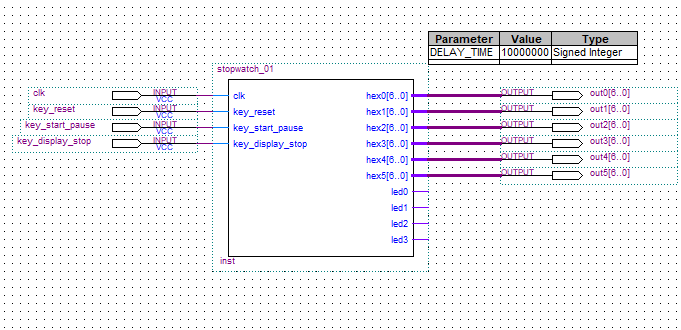
\includegraphics[width=\textwidth]{bdf.png}
            
        \subsection{verilog代码设计}
        	\par 详细请见代码注释。消抖的实现方式是记录之前的电位高低,随时与当前的电位高低对比,如果之前基本不是高电平,那么现在的低电平将不会导致状态的改变;现在的低电平只有在之前是高电平时才会改变计时与显示的状态。当然reset复位不受影响,因为从肉眼效果来看几次高频率的复位可以基本等效成1次复位。
        
    \section{具体步骤}
    
    	\subsection{初始化} 设备驱动安装、在新建设备时选择实验设备的型号、设置时钟脉冲频率等。
        
        \subsection{实现代码} 根据设计要求把代码的主要功能部分全部实现,在给出的代码中自己填写的主要包括
        \par 1) 具体的6位数字更改解决方案
        \par 2) 计时状态更改、显示状态更改、复位解决方案
        \par 3) 消抖解决方案
        \par 具体代码实现请看本实验报告的第4部分\emph{完整代码}
        
        \subsection{完成BDF设计} 根据实验要求把四个输入和六个输出分配好,用input和output的pin连接,以及保证基本的美观性和可读性。
        
        \subsection{针脚分配} 对于输入的button每个都有1个针脚,对于输出的数字每个都有7个针脚,按照实验手册进行匹配。
        \subsection{编译与写入} 把文件编译,写入开发板中。
    
    \section{完整代码}
    
    \par 注:由于latex排版代码不是很美观所以采用截图,如果需要完整代码,请至Github下载。地址https://github.com/yyong119/EI332SourceCode
    \par //****之中的注释是我认为比较关键的地方
 	\newline
    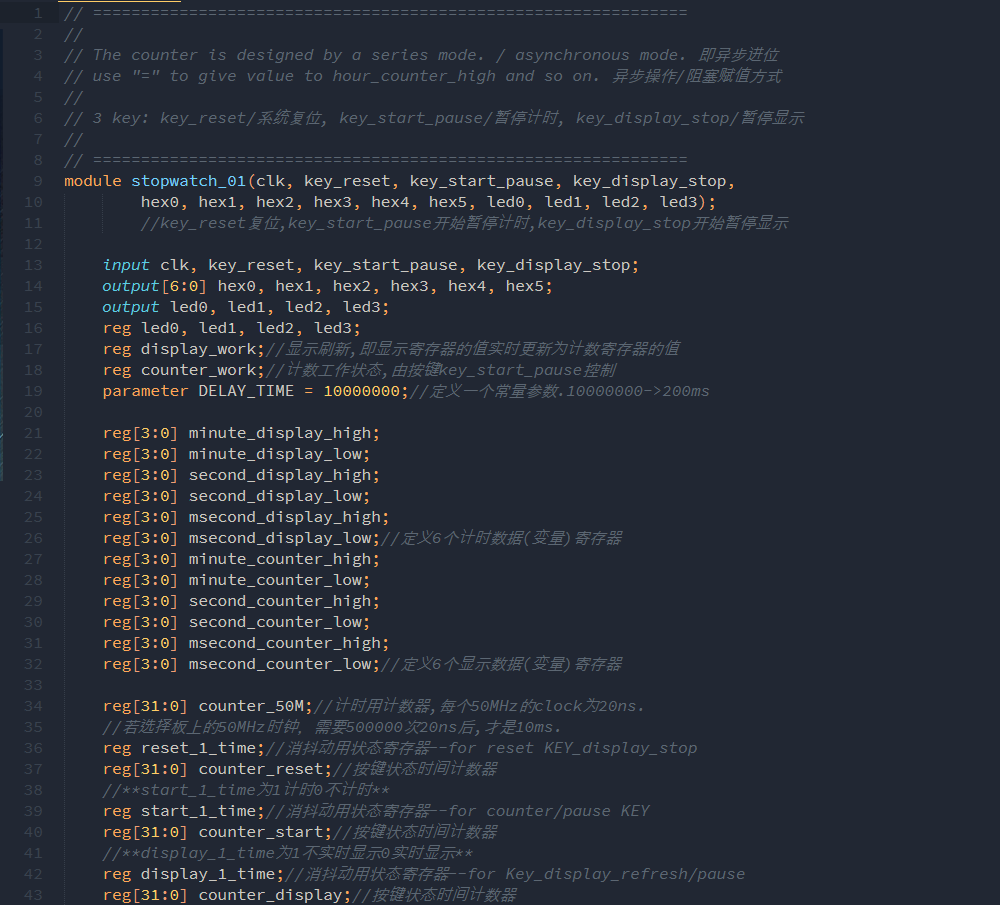
\includegraphics[width=\textwidth]{1-43.png}
    \newline
    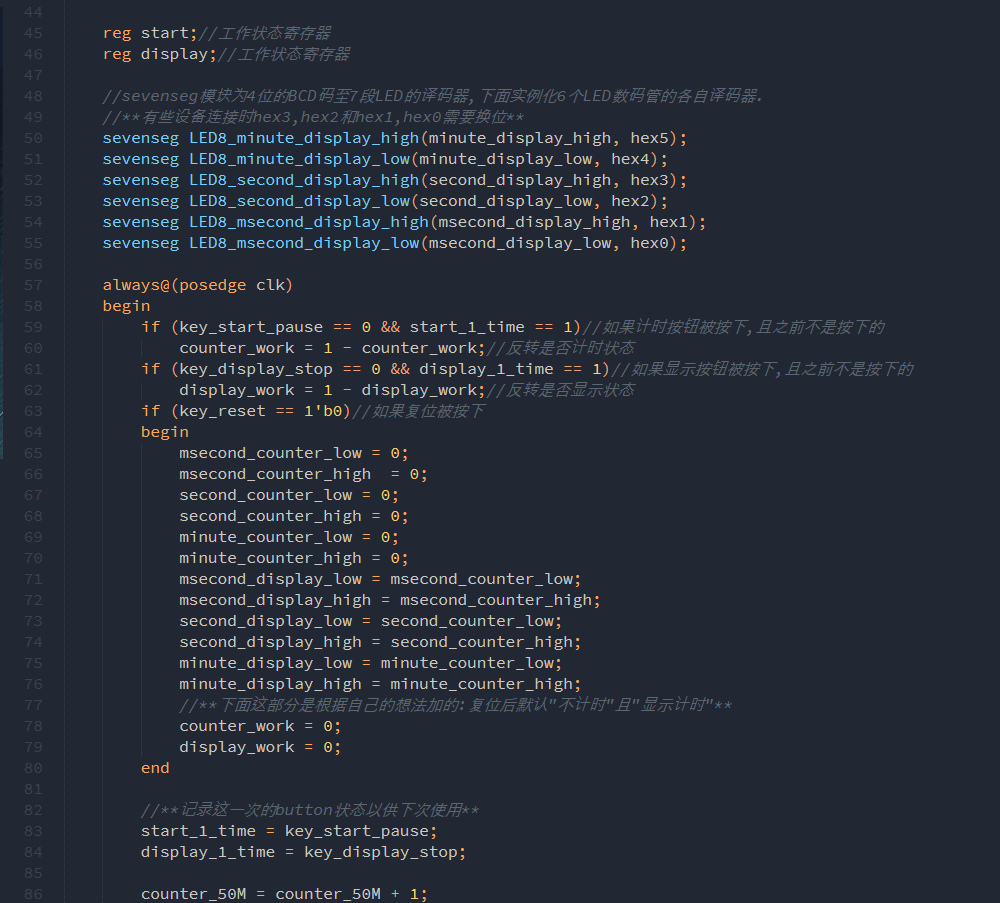
\includegraphics[width=\textwidth]{44-86.png}
    \newline
    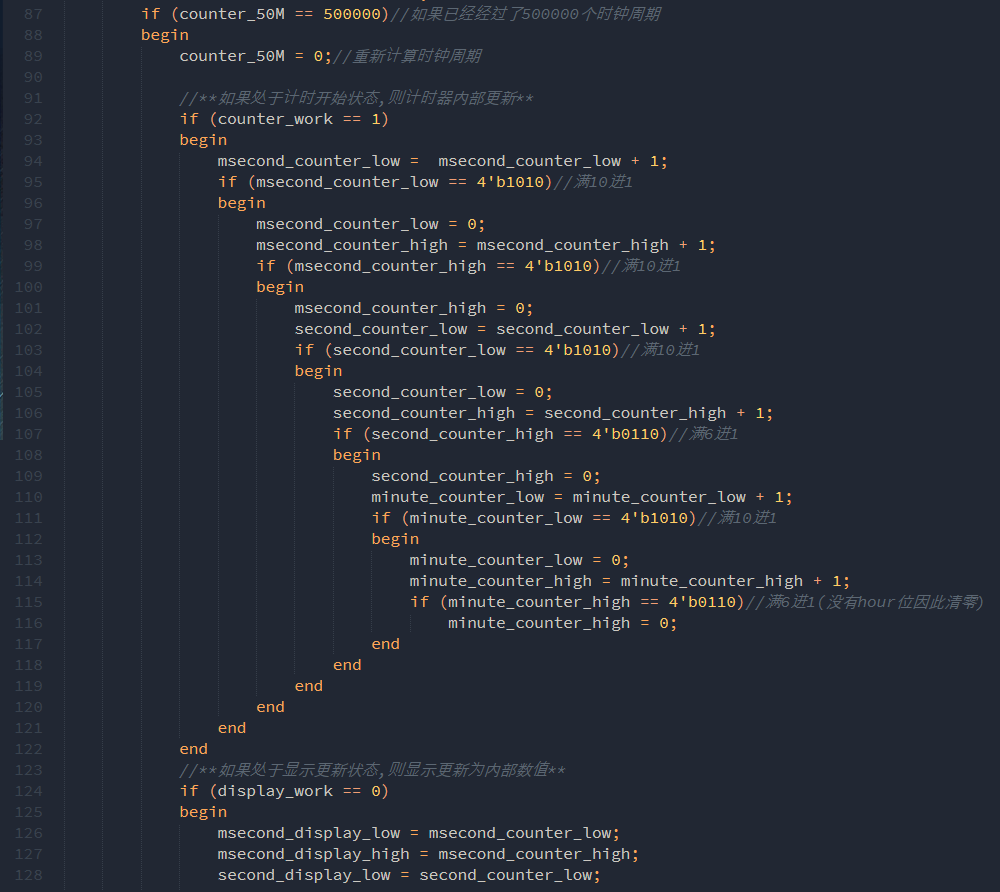
\includegraphics[width=\textwidth]{87-128.png}
    \newline
    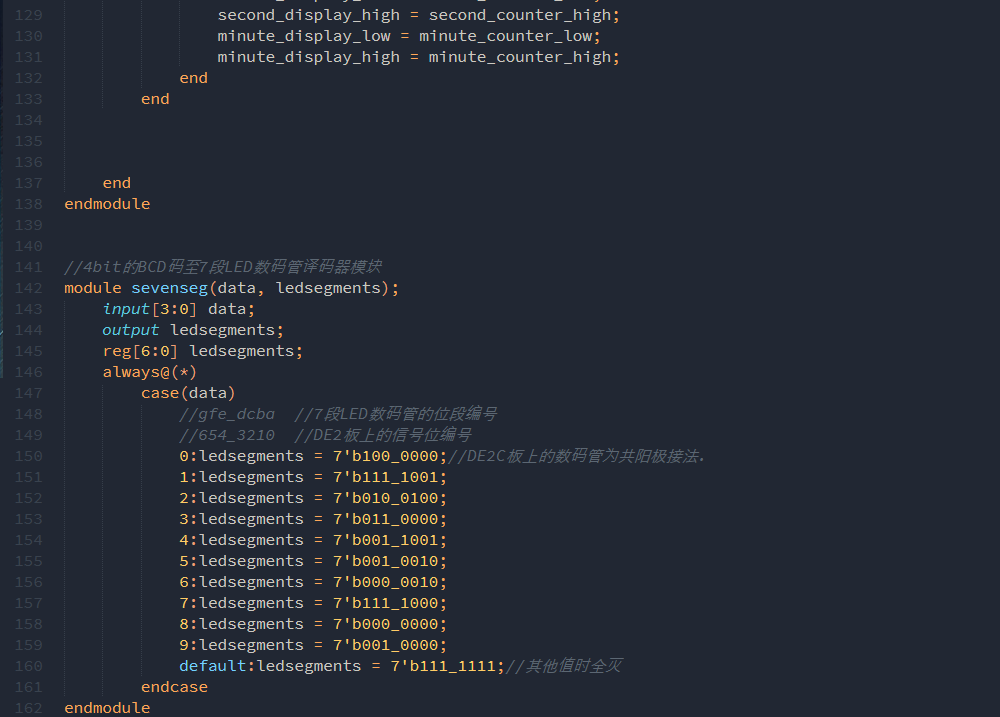
\includegraphics[width=\textwidth]{129-162.png}



\end{document}
